% Freer IA redshift evolution: the plan of the test and its results.
% Build with assets/build_note.sh of the summary-notes skill.
\documentclass[11pt]{article}

\usepackage[margin=1in]{geometry}
\usepackage{amsmath}
\usepackage{amssymb}
\usepackage{graphicx}
\usepackage{booktabs}
\usepackage{xcolor}
\usepackage[font=small,labelfont=bf,labelsep=period]{caption}
\usepackage[hidelinks]{hyperref}

\newcommand{\hMpc}{\,h\,{\rm Mpc}^{-1}}
\newcommand{\Om}{\Omega_{\rm m}}
\newcommand{\PNL}{P_{\rm NL}}

% =====================================================================
% Numbers
% =====================================================================
% Part 1: results. The statements of the Summary and of "Results" rest on them.
\newif\ifnumbersfinal
\numbersfinaltrue
\newcommand{\refresh}[1]{\ifnumbersfinal#1\else\textcolor{red}{#1}\fi}
% total MAP figure of bias, NLA, 3x2pt, xi cut 0.2, gamma_t 0.5, CMB prior
% (fisher_minimize.json, 3x2+cmb|NLA|0.2|S1|gt0.5 and |lin|gt0.5)
\newcommand{\FobS}{\refresh{0.28}}
\newcommand{\FobL}{\refresh{0.46}}
% the amplitude piece (bias_pieces.json, zshape "z|amplitude")
\newcommand{\AmpS}{\refresh{0.24}}
\newcommand{\AmpL}{\refresh{0.48}}
% the z = 3 snapshot alone (plots/amp_error/data.json, fob_snapshot)
\newcommand{\AmpThreeS}{\refresh{0.21}}
\newcommand{\AmpThreeL}{\refresh{0.40}}
% template check (fisher_minimize.py --check-hm): chi2(native - template) at A1 3.5, eta1 0.7
\newcommand{\TplCs}{0.009}
\newcommand{\TplTx}{0.010}
\newcommand{\TplSteepCs}{37}
\newcommand{\TplSteepTx}{51}
% TATT template check (fisher_minimize.py --check-tatt), at A1 3.4, eta1 0.7, A2 -1, eta2 -2, bTA 0.5:
% chi2(native - template); and g = 1.2: chi2 of the change, chi2(native - correction)
\newcommand{\TattTplCs}{0.011}
\newcommand{\TattTplTx}{0.011}
\newcommand{\TattGChgCs}{220}
\newcommand{\TattGChgTx}{171}
\newcommand{\TattGErrCs}{0.002}
\newcommand{\TattGErrTx}{0.001}
\newcommand{\TattAtwoNoBB}{0.5}   % relative norm of the A2-only mismatch without B modes
\newcommand{\TattDmax}{0.01}
\newcommand{\TattAtwoMax}{0.6}    % largest |A2| at the MAP of the 60 TATT freer-evolution fits (fisher_minimize.json)
\newcommand{\TattBtaMax}{0.17}    % largest b_TA, same      % largest |change| of the TATT figures of bias, first version to exact (tatt_exact)
% per-bin NLA (NLAz) in 3x2pt, rejected earlier (ia_error_budget.tex, "Freer redshift evolution")
\newcommand{\NLAzLo}{0.6}
\newcommand{\NLAzHi}{1.1}
% results (analysis/cut_validation/zevo_summary.json; fisher_minimize.json; bias_pieces.json),
% 3x2pt, gamma_t 0.5, w 0.2, CMB prior
\newcommand{\BkFobS}{\refresh{0.05}}      % NLAbk, S1, K0 = 0.2, total MAP
\newcommand{\HzFobS}{\refresh{0.03}}      % NLAhz, S1, K0 = 0.2
\newcommand{\BkAmpS}{\refresh{0.05}}      % NLAbk, S1, K0 = 0.2, amplitude piece
\newcommand{\HzAmpS}{\refresh{0.02}}
\newcommand{\BkAmpL}{\refresh{0.13}}      % lin
\newcommand{\HzAmpL}{\refresh{0.03}}
\newcommand{\ChiNLA}{\refresh{1.24}}      % chi2 at the MAP, S1, K0 = 0.2 (noiseless data: the misfit)
\newcommand{\ChiBk}{\refresh{0.21}}
\newcommand{\ChiHz}{\refresh{0.20}}
\newcommand{\EtaNLA}{\refresh{0.83}}      % eta1, S1, K0 = 0.2
\newcommand{\EtaBk}{\refresh{0.71}}
\newcommand{\DetaS}{\refresh{0.38 to 0.43}}  % NLAbk Delta eta, S1 and EB, all K0
\newcommand{\DetaL}{\refresh{0.49 to 0.52}}  % lin
\newcommand{\GthreeS}{\refresh{1.21}}     % g(3) of both families, S1
\newcommand{\GthreeL}{\refresh{1.27 to 1.31}} % lin
\newcommand{\IIhiS}{\refresh{0.22 to 0.25}}  % largest piece (II, k > 0.3) of NLAbk/NLAhz, S1, K0 0.4 to 0.6
\newcommand{\IIlinThree}{\refresh{0.18}}  % largest piece (II, 0.06 to 0.3), lin, K0 = 0.3
\newcommand{\IIlinFour}{\refresh{0.43}}   % same at K0 = 0.4
\newcommand{\SigNLA}{\refresh{0.0044}}    % sigma(S8), NLA, K0 = 0.2
\newcommand{\SigBkTwo}{\refresh{0.0045}}  % NLAbk, K0 = 0.2
\newcommand{\SigBkSix}{\refresh{0.0032}}  % NLAbk, K0 = 0.6
\newcommand{\SigBkLin}{\refresh{0.0041}}  % NLAbk, K0 = 0.3
\newcommand{\NFits}{134}
% Part 2: inputs.
\newcommand{\Zb}{1.5}
\newcommand{\Tol}{0.3}

\begin{document}

\begin{center}
  {\LARGE Freer IA redshift evolution: plan and results\par}
  \vspace{0.6em}
  {\large Does a redshift model freer than $(1+z)^{\eta_1}$ remove the amplitude floor of NLA and TATT?\par}
  \vspace{0.6em}
  {\large November 2026\par}
\end{center}
\vspace{1em}

\section{Summary}

\paragraph{The question.}
In the every-parameter-free cut validation (notes/ia\_error\_budget), the
bias of NLA in 3x2pt has a floor that no scale cut removes: the
redshift-amplitude piece, the error of the power law $A_1(z) = A_1
[(1+z)/1.62]^{\eta_1}$ against FLAMINGO's amplitude at each snapshot. It is
\AmpS$\sigma$ of the total \FobS$\sigma$ on the stitched truth and \AmpL$\sigma$
of \FobL$\sigma$ on the linear-limit truth ($\xi_\pm$ cut 0.2, $\gamma_t$ cut
0.5; the pieces are linear shifts and partly cancel, so one can exceed the
total). The test asks whether a freer, nested redshift model removes it, and at
what cost in constraining power.

\paragraph{The answer.}
Yes. One extra parameter, a change of slope above $z = \Zb$, removes the
floor: the amplitude piece falls from \AmpS{} to \BkAmpS{} (stitched) and
from \AmpL{} to \BkAmpL{} (linear limit), the total from \FobS{} to
\BkFobS. The 3x2pt reliable cut of NLA rises from 0.2 to 0.6 or beyond
(the end of the grid) on the stitched and E minus B truths, and from none
to 0.3 on the linear-limit truth; $\sigma(S_8)$ at the reliable cut falls
from \SigNLA{} to \SigBkSix. The extra parameter costs about 2\% in
$\sigma(S_8)$ at a fixed cut. Free amplitudes at $z = 2$ and 3 give the
same, and TATT with the break behaves as NLA with it. What limits the cut
next is the scale dependence of II, not the redshift evolution
(Section~\ref{sec:results}).

\paragraph{Where the floor comes from.}
Split by snapshot, the amplitude piece is almost entirely the $z = 3$
snapshot: \AmpThreeS$\sigma$ of \AmpS{} (stitched) and \AmpThreeL$\sigma$ of
\AmpL{} (linear limit); every snapshot at $z \le 1$ gives at most
$0.02\sigma$ (Figure~\ref{fig:amp}). The fitted power law falls short of
FLAMINGO there by 10 to 12\% in GI and 18 to 32\% in II. The freedom the
test adds is therefore above $z = \Zb$.

\paragraph{The models.}
Two families, each nested in the power law ($g = 1$ is NLA or TATT):
a slope break above $z = \Zb$ (one parameter) and free amplitudes at $z = 2$
and 3 (two parameters), for NLA and for TATT: NLAbk, NLAhz, TATTbk, TATThz.

\paragraph{The runs.}
The protocol of the note: total MAP figure of bias and the bias split, cosmic
shear at $K_0 = 0.2$ to 0.5 and 3x2pt at $K_0 = 0.2$ to 0.6 with $\gamma_t$
at 0.5 and $w$ at 0.2, on the stitched, E minus B and linear-limit truths,
with NLA and TATT at the same cuts: \NFits{} fits.

\section{Why per-bin amplitudes are not the test}
cosmolike's per-bin mode (NLAz: one amplitude per source bin) was tried in
the note. In cosmic shear it follows the power law to 7\% in bins 1 to 7; in
3x2pt it holds the amplitude constant across a source bin, which drops the
evolution inside the bin that $\gamma_t$ sees where sources overlap lenses,
and it fits FLAMINGO worse than NLA even at fixed cosmology (figures of bias
\NLAzLo{} to \NLAzHi, not counted). The valid test keeps the power law
inside every bin and adds freedom on top of it, as a function of $z$.

\section{The models}
\label{sec:models}
Each model multiplies the alignment amplitudes by a common factor $g(z)$:
\begin{equation}
  a_1(z) = A_1 \left(\frac{1+z}{1.62}\right)^{\eta_1} g(z), \qquad
  a_2(z) = A_2 \left(\frac{1+z}{1.62}\right)^{\eta_2} g(z),
\end{equation}
with $b_{\rm TA}$ unchanged ($A_2 = b_{\rm TA} = 0$ for NLA). A common
factor treats the departure from the power law as a change of the whole
alignment signal of the sample, so every TATT term that carries $a_1$ or
$a_2$, the $a_1 b_{\rm TA}$ and $a_1 a_2$ terms included, moves with it.
\begin{description}
  \item[Break (NLAbk, TATTbk).] The slope changes by $\Delta\eta$ above
    $z_b = \Zb$:
    \begin{equation}
      g(z) = \left(\frac{1+z}{1+z_b}\right)^{\Delta\eta} \ (z > z_b), \qquad g = 1 \ (z \le z_b),
    \end{equation}
    with $\Delta\eta$ flat in $[-5, 5]$. One parameter; continuous at $z_b$.
  \item[High-$z$ amplitudes (NLAhz, TATThz).] Free amplitudes at $z = 2$ and 3:
    \begin{equation}
      g(z) = 1 + d_2\, T_2(z) + d_3\, T_3(z),
    \end{equation}
    $T_2$ the tent on $z = 1.5, 2, 3$ and $T_3$ rising from 0 at $z = 2$ to 1
    at $z = 3$, held at its $z = 3$ value beyond; $d_2, d_3$ flat in
    $[-0.9, 3]$ ($g > 0$). Two parameters; it can follow a rise and a
    flattening that a slope cannot.
\end{description}
The break is the minimal extension that the amplitude split asks for; the
high-$z$ amplitudes test whether the $z = 3$ error is a smooth trend or one
outlying snapshot. Figure~\ref{fig:amp} (bottom) shows both at example values.

\begin{figure}[t]
  \centering
  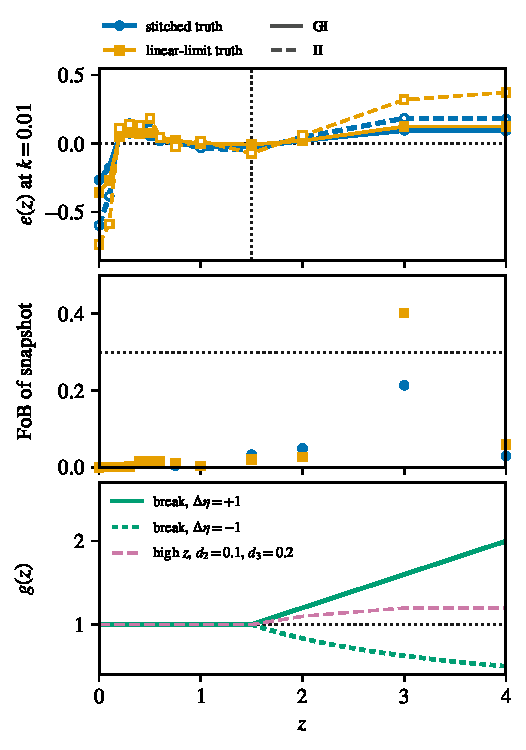
\includegraphics[width=0.62\textwidth]{plots/amp_error/amp_error.pdf}
  \caption{Top: the amplitude error of NLA at each FLAMINGO snapshot,
    $\epsilon = 1 - P^{\rm model}/P^{\rm truth}$ at $k = 0.01\hMpc$ (GI solid,
    filled; II dashed, open), of the 3x2pt fit at $\xi_\pm$ cut 0.2 and
    $\gamma_t$ cut 0.5, on the stitched and linear-limit truths. Middle: the
    figure of bias of each snapshot's amplitude error alone, against the
    \Tol$\sigma$ tolerance (dotted). Bottom: $g(z)$ of the two freer models
    at example values; the dotted vertical line is $z = \Zb$.}
  \label{fig:amp}
\end{figure}

\section{Implementation}
\paragraph{Templates.}
The data vector is linear in the IA spectra. Every GI term of TATT is
linear in $(a_1, a_2)$ and every II term quadratic, so at snapshot $s$ the
common factor changes GI by $(g_s - 1)$ and II by $(g_s^2 - 1)$ times its
native value:
\begin{equation}
  v \to v + \sum_s (g_s - 1)\, {\rm GI}_s + (g_s^2 - 1)\, {\rm II}_s,
\end{equation}
with the $\gamma_t$ rows scaled by $b_i/b_i^{\rm fid}$, as for the
halo-model correction. ${\rm GI}_s$ and ${\rm II}_s$ are the native TATT
parts at the power-law amplitudes, built from per-term snapshot templates
(tatt\_templates.py): the data-vector response, on the base of the note, of
each amplitude product at unit coefficient, three for GI ($a_1$,
$a_1 b_{\rm TA}$, $a_2$) and six for II ($a_1^2$, $a_1^2 b_{\rm TA}$,
$a_1^2 b_{\rm TA}^2$, $a_1 a_2$, $a_1 a_2 b_{\rm TA}$, $a_2^2$), the last
three with their B modes, which enter $\xi_+$ as the E modes do and $\xi_-$
with the opposite sign. For NLA only the $a_1$ and $a_1^2$ rows act; they
equal the native-NLA templates of hm\_templates.py to $10^{-6}$. The extra parameters are not cosmolike parameters;
the minimizer removes them before the likelihood call.
(fisher\_minimize.py: \texttt{ZEVO}, \texttt{zevo\_g},
\texttt{Setup.tatt\_parts}, \texttt{Setup.zevo\_correction}; bias\_pieces.py:
\texttt{model\_ratios}, where the model's $P_{GI}$ is multiplied by $g_s$ and
$P_{II}$ by $g_s^2$.)

\paragraph{Checks done.}
\begin{itemize}
  \item With the extra parameters at zero both models reproduce NLA exactly
    (maximum difference 0 on the 3x2pt vector).
  \item The template sum reproduces the native NLA at $A_1 = 3.5$,
    $\eta_1 = 0.7$ to $\chi^2 = \TplCs$ (cosmic shear) and \TplTx{} (3x2pt)
    of the difference. For a steep evolution, $\eta_1 = 2$, it degrades to
    $\chi^2 = \TplSteepCs$ and \TplSteepTx: between the sparse high-$z$
    snapshots (1.5, 2, 3, 4) the templates interpolate the tables linearly,
    while cosmolike evaluates the power law at every $z$. A fit that drives
    $g$ far from 1 is flagged for this reason.
  \item The TATT template sum reproduces cosmolike's native TATT at
    $A_1 = 3.4$, $\eta_1 = 0.7$, $A_2 = -1$, $\eta_2 = -2$, $b_{\rm TA} = 0.5$
    to $\chi^2 = \TattTplCs$ (cosmic shear) and \TattTplTx{} (3x2pt). A
    constant $g = 1.2$ is the same as native TATT at $1.2 A_1$ and $1.2 A_2$:
    the correction reproduces that change ($\chi^2 = \TattGChgCs$ and
    \TattGChgTx) to $\chi^2 = \TattGErrCs$ and \TattGErrTx. Without the B modes
    the $a_2$-only part misses the native vector by half its norm
    (\TattAtwoNoBB); with them, by 2 to 3\%.
  \item The fitted amplitudes stay near $A_1 \simeq 3.4$, $\eta_1 \simeq 0.7$,
    where the templates are accurate; the steep case above is the same for
    NLA and TATT, a limit of the snapshot base, not of the TATT terms.
\end{itemize}

\paragraph{Approximation.}
The correction is held at the fiducial cosmology (D3A); the native part
responds fully. The same approximation is used for the halo-model models in
the note.

\paragraph{First version of the TATT variants.}
The first TATT runs moved only the terms of NLA form with $g$ ($a_1 P_{\rm
NL}$ in GI, $a_1^2 P_{\rm NL}$ in II) and left the $a_1 b_{\rm TA}$,
$a_1 a_2$ and $a_2$ terms on the power law. All 60 TATT fits were rerun with
the common factor of Section~\ref{sec:models}. The figures of bias change by
at most \TattDmax{} (Figure~\ref{fig:tattexact}) and no reliable cut moves:
at the MAP, $|A_2| \le \TattAtwoMax$ and $b_{\rm TA} \le \TattBtaMax$
(the largest values on the linear-limit truth), so the terms the first
version missed carry little of the signal.

\begin{figure}[!htbp]
  \centering
  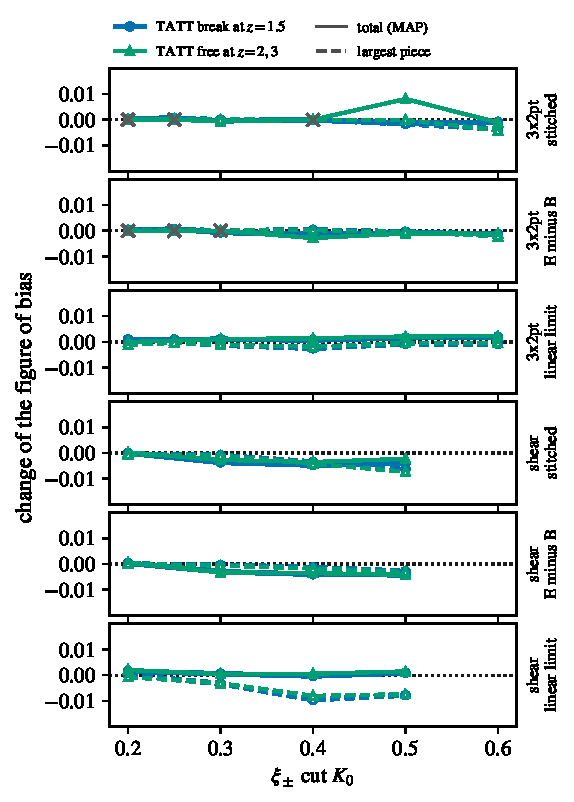
\includegraphics[width=0.5\textwidth]{plots/tatt_exact/tatt_exact.pdf}
  \caption{Change of the TATT figures of bias from the first version ($g$ on
    the NLA-form terms only) to the common factor on $a_1$ and $a_2$ in every
    term, against the $\xi_\pm$ cut, per probe and truth (3x2pt: $\gamma_t$
    0.5, $w$ 0.2). Solid, filled: the total MAP figure of bias; dashed, open:
    the largest piece of the bias split. A grey cross marks a fit with
    $\eta_2$ at its bound. The dotted line is zero.}
  \label{fig:tattexact}
\end{figure}

\section{Runs}
\begin{center}
\begin{tabular}{lll}
  \toprule
  probe & cuts & per model and truth \\
  \midrule
  cosmic shear + CMB prior & $K_0 = 0.2, 0.3, 0.4, 0.5$ & 4 fits \\
  3x2pt + CMB prior, $\gamma_t$ 0.5, $w$ 0.2 & $K_0 = 0.2, 0.25, 0.3, 0.4, 0.5, 0.6$ & 6 fits \\
  \bottomrule
\end{tabular}
\end{center}
Four models and three truths (stitched, E minus B, linear limit) give 120
fits; with the NLA and TATT runs that did not yet exist at these cuts,
\NFits{} were run, each followed by its bias split. The 3x2pt grid first
stopped at 0.4 and was extended to 0.6 when the freer models still passed
there. The fits ran two at a time at the lowest priority on the M3 Mac.

\section{What the results are judged by}
\begin{enumerate}
  \item \textbf{Physical fit.} No parameter within 2\% of its prior range
    of a bound; the fitted $g$ follows the amplitude error it is meant to
    absorb: on the stitched truth $g(3) \simeq 1.1$ ($\Delta\eta \simeq
    0.2$), on the linear-limit truth 1.15 to 1.2.
  \item \textbf{The floor.} The amplitude piece of the bias split, against
    \AmpS$\sigma$ and \AmpL$\sigma$ of NLA. The models do what they are for
    if it falls well below \Tol$\sigma$ on every truth.
  \item \textbf{The reliable cut.} The criterion of the note (total MAP
    figure of bias and every piece below \Tol$\sigma$ at the cut and every
    smaller cut with a physical fit), per model and truth, against NLA and
    TATT at the same cuts.
  \item \textbf{The cost.} $\sigma(S_8)$ and the figure of merit against NLA
    and TATT at the same cut, and at each model's own reliable cut: a freer
    model is worth it only if the higher cut it allows gains more than its
    extra parameters cost.
  \item \textbf{Consistency.} The same conclusion on the stitched and E minus
    B truths, and the direction of the linear-limit truth, whose large scales
    come from the measured points.
\end{enumerate}

\section{Results}
\label{sec:results}

\paragraph{3x2pt.}
Figure~\ref{fig:nla} shows NLA and its two freer evolutions, Figure~\ref{fig:tatt}
TATT. With the power law, the total and the amplitude piece exceed
\Tol$\sigma$ from $K_0 = 0.25$ to 0.3 on the stitched and E minus B truths and
at every cut on the linear-limit truth. With the break or the high-$z$
amplitudes, the total stays at 0.02 to 0.09 up to $K_0 = 0.6$ on the stitched
and E minus B truths, and the amplitude piece at \BkAmpS{} and \HzAmpS{}
(stitched, $K_0 = 0.2$). The largest piece left is the scale dependence of
II: above $k = 0.3\hMpc$ on the stitched truth (\IIhiS{} at $K_0 = 0.4$ to
0.6, below the tolerance), and at 0.06 to $0.3\hMpc$ on the linear-limit
truth (\IIlinThree{} at $K_0 = 0.3$, \IIlinFour{} at 0.4), which sets that
truth's cut at 0.3.

\begin{figure}[t]
  \centering
  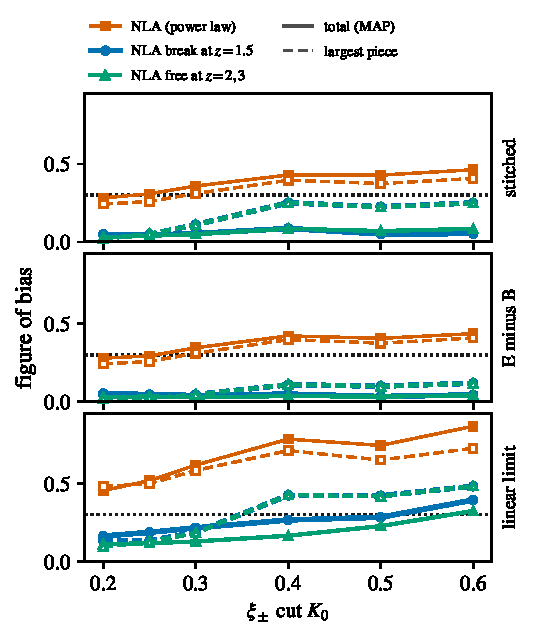
\includegraphics[width=0.62\textwidth]{plots/zevo_3x2_nla/zevo_3x2_nla.pdf}
  \caption{The 3x2pt figure of bias against the $\xi_\pm$ cut ($\gamma_t$ cut
    0.5, $w$ cut 0.2, every parameter free, CMB prior), one panel per truth:
    NLA with the power law, with a slope break at $z = 1.5$, and with free
    amplitudes at $z = 2$ and 3. Solid, filled: the total MAP figure of bias;
    dashed, open: the largest piece of the bias split. The dotted line is the
    \Tol$\sigma$ tolerance.}
  \label{fig:nla}
\end{figure}

\begin{figure}[t]
  \centering
  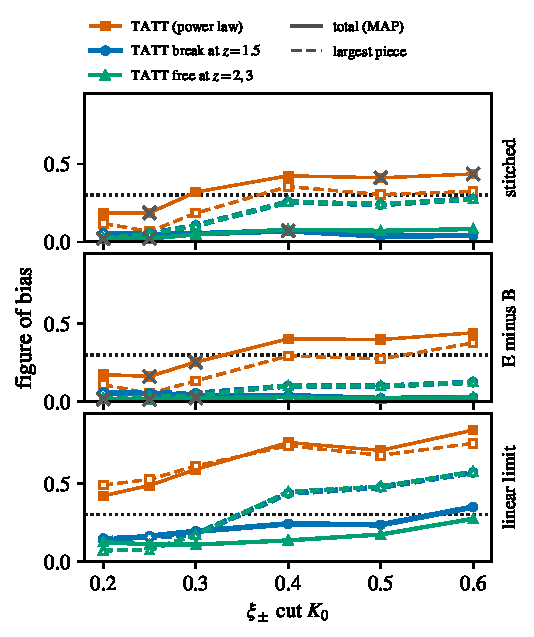
\includegraphics[width=0.62\textwidth]{plots/zevo_3x2_tatt/zevo_3x2_tatt.pdf}
  \caption{As Figure~\ref{fig:nla}, for TATT. A grey cross marks a fit with a
    parameter at a prior bound ($\eta_2$ within 2\% of $\pm 5$), which the
    reliable cut does not use.}
  \label{fig:tatt}
\end{figure}

\paragraph{Reliable cuts and cost.}
The criterion of the note (total and every piece below \Tol$\sigma$, there
and at every smaller cut with a physical fit):
\begin{center}
\begin{tabular}{lccc}
  \toprule
  3x2pt model & stitched & E minus B & linear limit \\
  \midrule
  NLA & 0.2 & 0.25 & none \\
  NLA, break & $\ge 0.6$ & $\ge 0.6$ & 0.3 \\
  NLA, high-$z$ amplitudes & $\ge 0.6$ & $\ge 0.6$ & 0.3 \\
  TATT & 0.2 & 0.2 & none \\
  TATT, break & $\ge 0.6$ & $\ge 0.6$ & 0.3 \\
  TATT, high-$z$ amplitudes & $\ge 0.6^{a}$ & $\ge 0.6^{a}$ & 0.3 \\
  \bottomrule
\end{tabular}

\smallskip
{\footnotesize $^{a}$ $\eta_2$ at its bound at $K_0 \le 0.25$ (stitched) and
$\le 0.3$ (E minus B); the cut rests on the physical fits above.}
\end{center}
At a fixed cut the extra parameter costs little: $\sigma(S_8) =
\SigBkTwo$ for NLA with the break at $K_0 = 0.2$ against \SigNLA{} for NLA.
At the reliable cut it gains: \SigBkSix{} at $K_0 = 0.6$ against \SigNLA{}
at 0.2, 27\% smaller (and \SigBkLin{} at 0.3 on the linear-limit truth,
where NLA has no passing cut).

\paragraph{The fits are physical.}
No parameter of the NLA variants sits at a bound. The break steepens the
slope above $z = 1.5$ by $\Delta\eta = \DetaS$ (stitched and E minus B) and
\DetaL{} (linear limit), stable across the cuts, while $\eta_1$ below it
falls from \EtaNLA{} to \EtaBk: with the high redshifts freed, the power law
follows $z < 1.5$ instead of compromising. The two families agree on the
amplitude at $z = 3$: $g(3) = \GthreeS$ on the stitched truth and \GthreeL{}
on the linear-limit truth. This is larger than the plan's estimate from the
power law's own error ($\simeq 1.1$), because $\eta_1$ refits lower at the
same time. The misfit $\chi^2$ at the MAP (noiseless data) falls from
\ChiNLA{} to \ChiBk{} and \ChiHz. TATT with the high-$z$ amplitudes puts
$\eta_2$ at $-5$ at the smallest cuts, where $A_2 \simeq 0.1$ leaves it
unconstrained; TATT with the break has no parameter at a bound.

\paragraph{Cosmic shear.}
Cosmic shear alone is not limited by the redshift evolution: the reliable
cut is 0.3 (stitched) and 0.5 (E minus B, the end of its grid) for every
model except TATT with the high-$z$ amplitudes, which reaches 0.5 on the
stitched truth too. On the
linear-limit truth it rises from none to 0.2 with any freer evolution.

\section{Open issues}
\begin{itemize}
  \item The $z = 3$ snapshot that carries the floor is also where the
    FLAMINGO alignment amplitude is lowest relative to TNG300 (ratio 0.53 in
    the same stellar-mass range); a freer model that absorbs it is fitting the
    least certain snapshot of the truth.
  \item The 3x2pt runs use $\gamma_t$ at 0.5 and $w$ at 0.2, the protocol of
    the IA note. With FLAMINGO's nonlinear galaxy bias in the data that pair
    fails, and the $\gamma_t$ and $w$ cuts are set per lens bin instead
    (IA note, Section ``Nonlinear galaxy bias''); the freer models were not
    rerun at those cuts.
  \item The grid ends at $K_0 = 0.6$, where the freer models still pass on
    the stitched and E minus B truths; their limit there is not found.
  \item The $\gamma_t$ and $w$ cuts were not raised with the freer models;
    whether they could be is not tested here.
\end{itemize}

\end{document}
